\section{Additional figure}\label{S1A1}


\begin{figure}[!htbp]
\centering
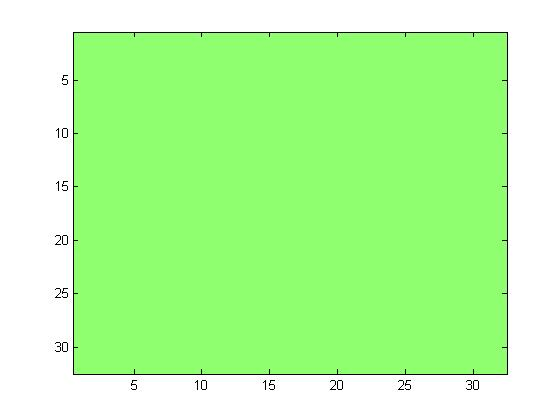
\includegraphics[width=1\textwidth]{6.jpg}
\subcaption{Time domain components}
\end{figure}

\begin{figure}[!htbp]
\centering
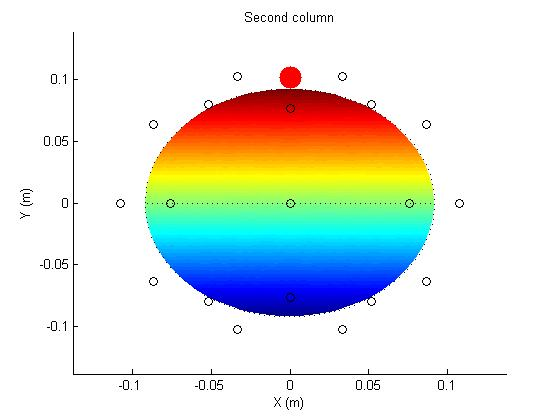
\includegraphics[width=1\textwidth]{7.jpg}
\caption{}
\end{figure}






\begin{figure}[!htbp]
\minipage{.5\textwidth}%
\centering
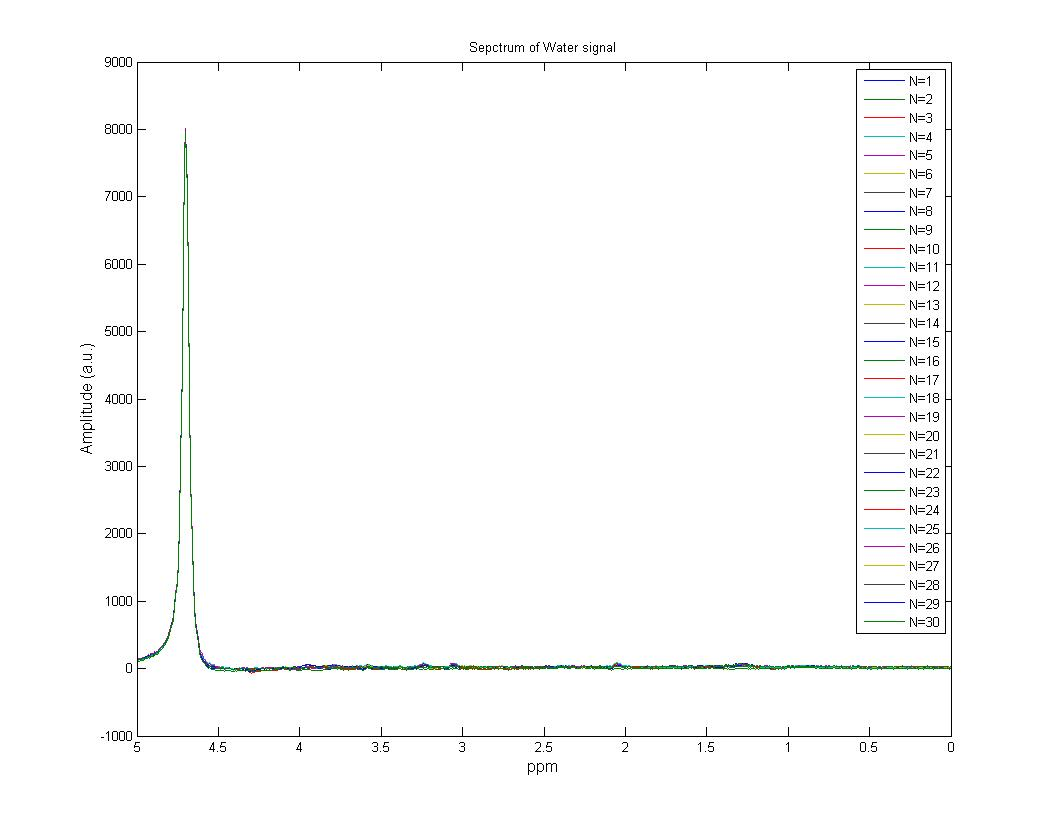
\includegraphics[width=1\textwidth]{9.jpg}
\subcaption{Spectrum water signal for different order model}\label{fig5}
\endminipage\hfill
\minipage{.5\textwidth}%
\centering
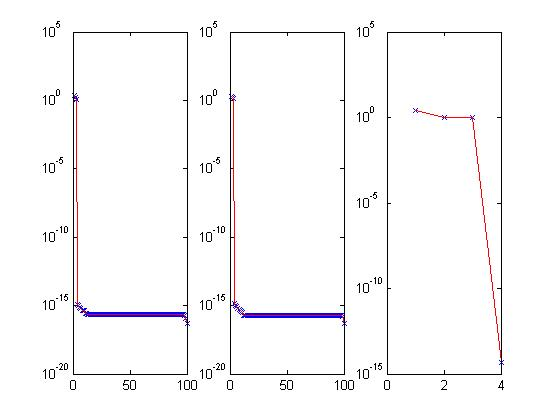
\includegraphics[width=1\textwidth]{10.jpg}
\subcaption{Water signal in time domain for different order model}\label{fig4}
\endminipage\hfill
\caption{}
\end{figure}

\begin{figure}[!htbp]
\centering
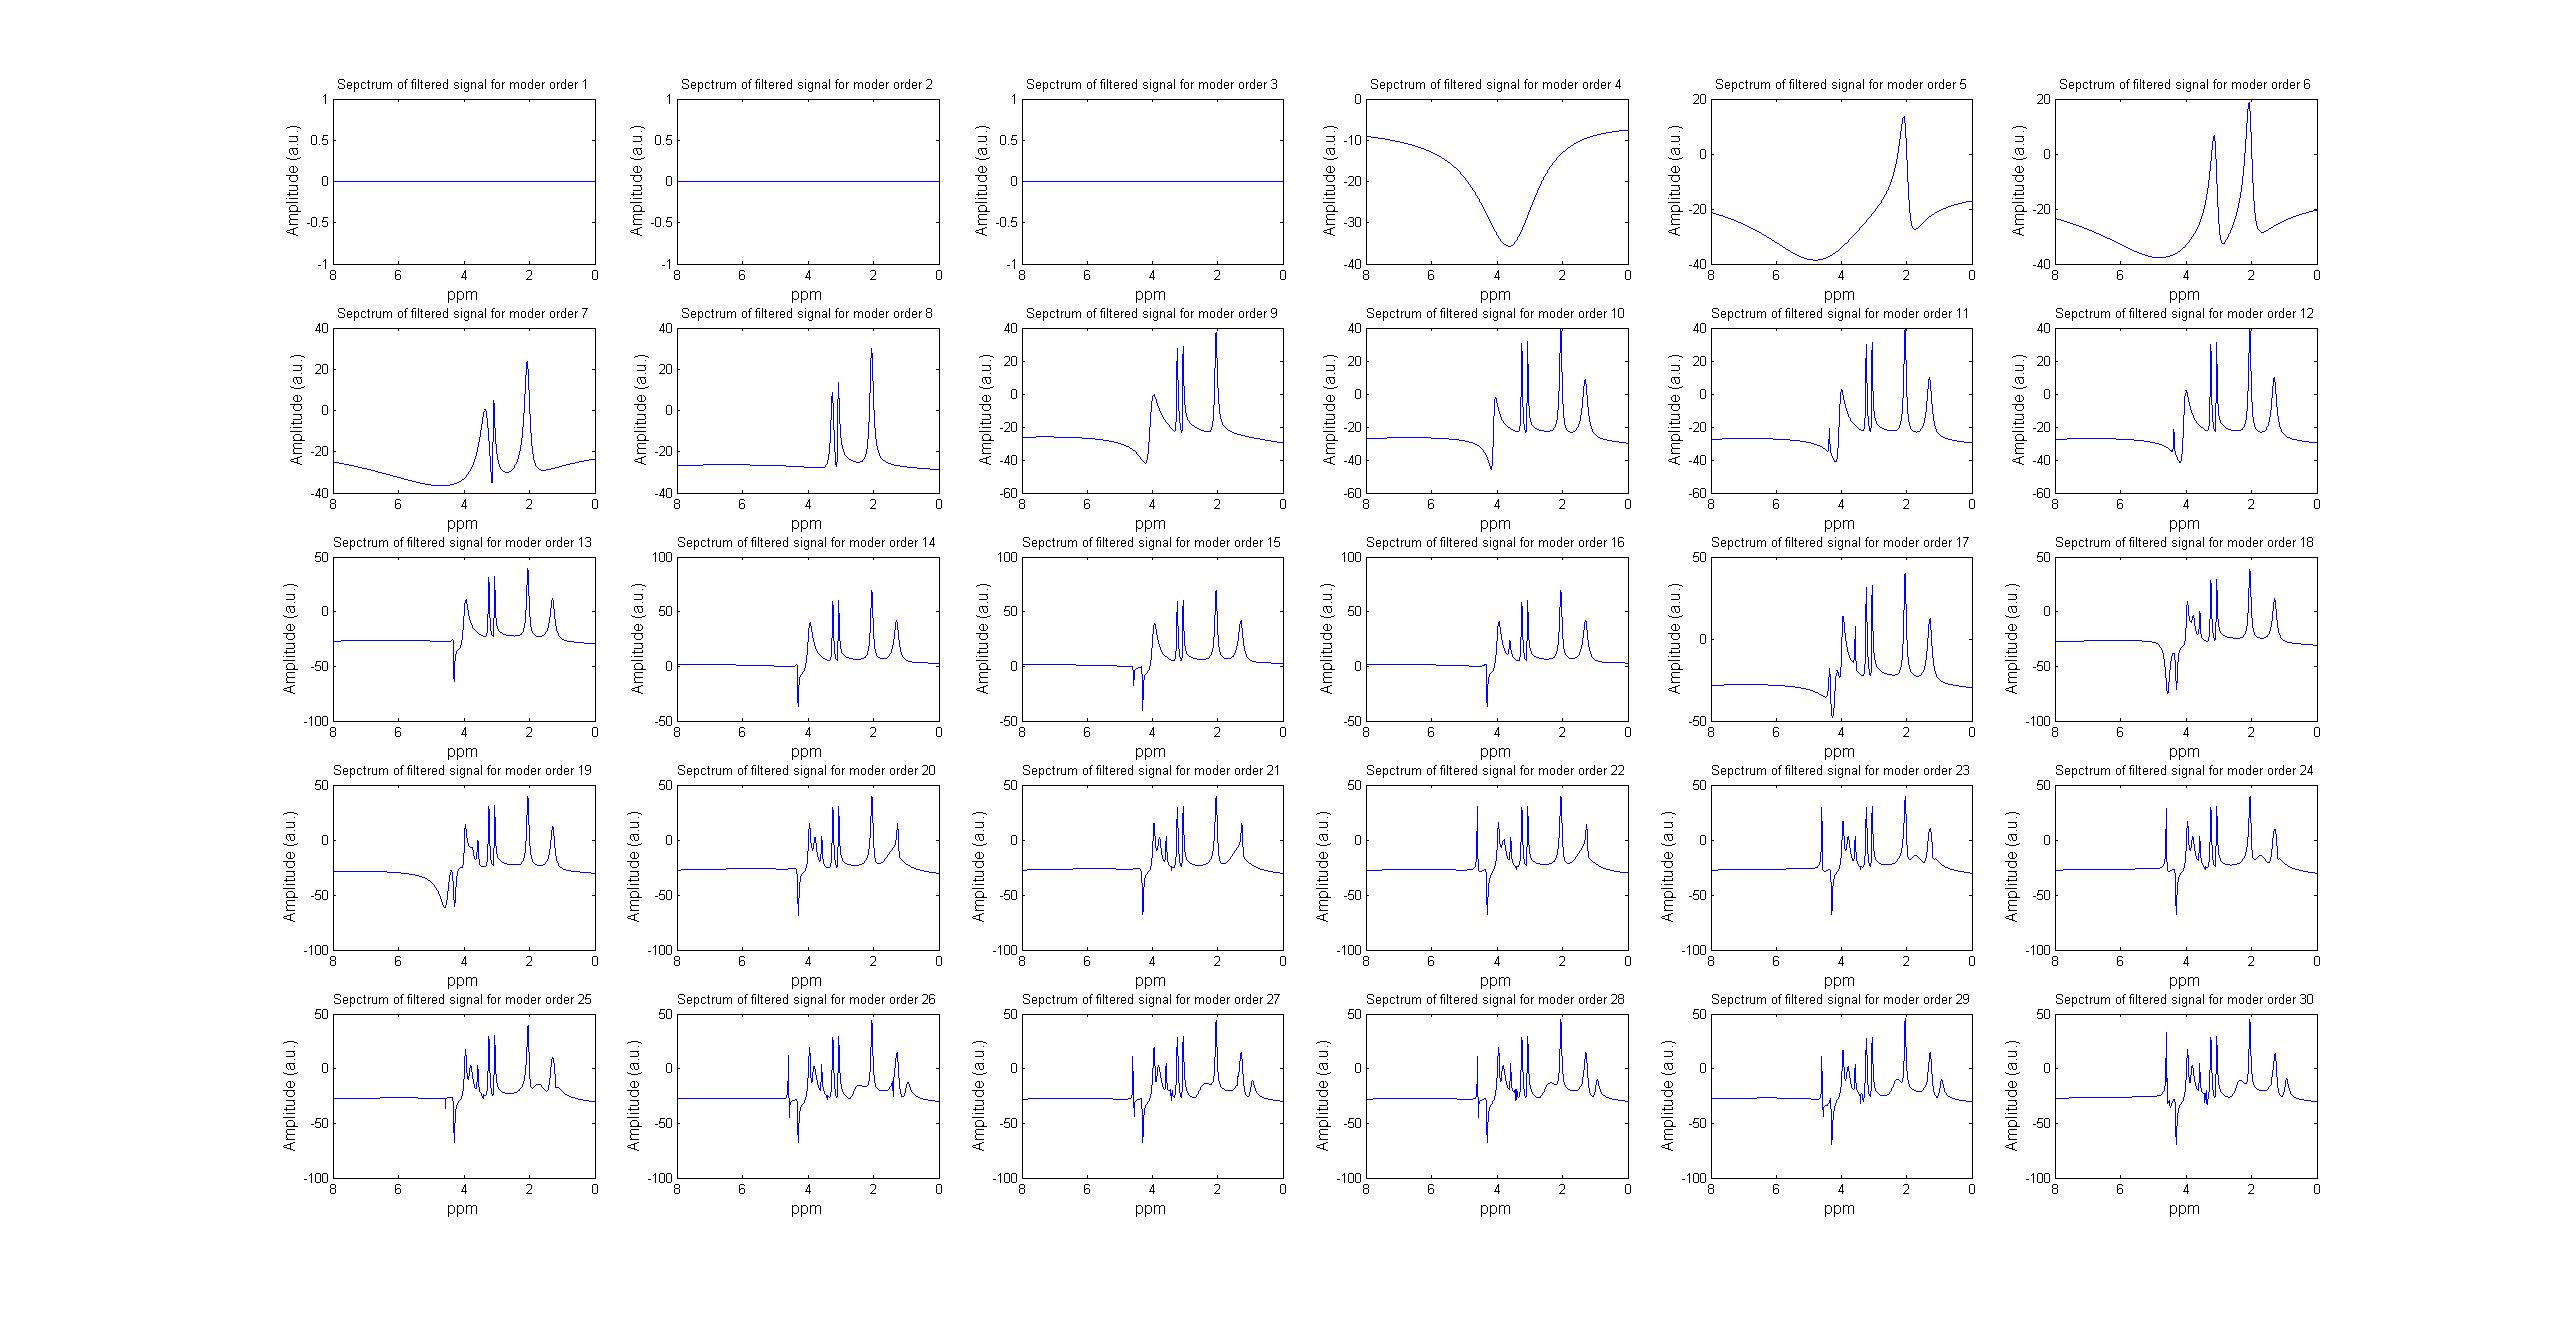
\includegraphics[width=1\textwidth]{8_2.jpg}
\caption{Spectrum Water filtered signal for different order model}\label{fig6}
\end{figure}

\begin{figure}[!htbp]
\centering
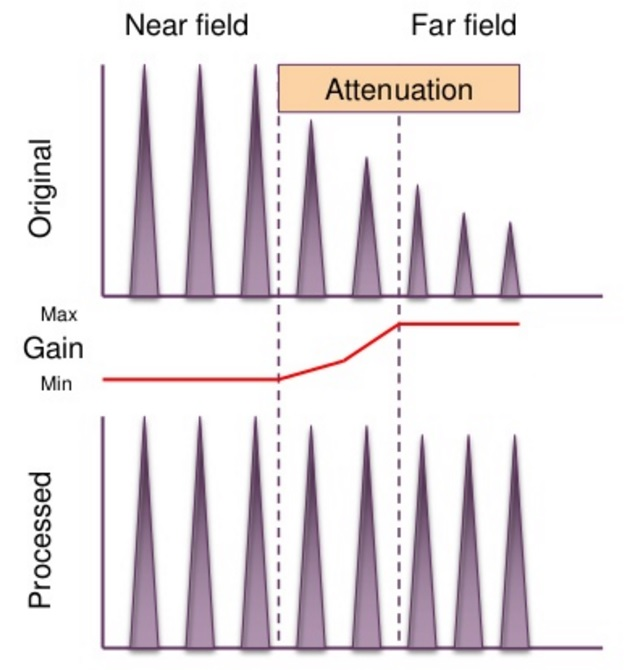
\includegraphics[width=1\textwidth]{8.jpg}
\caption{Spectrum Water filtered signal for different order model}\label{fig7}
\end{figure}




\begin{equation}\label{eq1}
y(t)=\sum_{k=1}^{K} a_{k}exp(j\phi_{k})exp(-d_{k}t+2\pi f_{k}t)\delta t
\end{equation}

\begin{equation}
ppm=\frac{f_{Hz}*10^6}{f_{s}}-ppm_{Ref}
\end{equation}